\documentclass{standalone}
\usepackage{tikz}
\usepackage{ctex,siunitx}
\setCJKmainfont{Noto Serif CJK SC}
\usepackage{tkz-euclide}
\usepackage{amsmath}
\usetikzlibrary{patterns, calc,3d}
\usetikzlibrary {decorations.pathmorphing,decorations.pathreplacing,decorations.shapes}
% \tikzset{
%   every node/.style={circle,thick,draw=red!50!black,fill=red!20!white,minimum height=7mm}
% }
\begin{document}
\Large
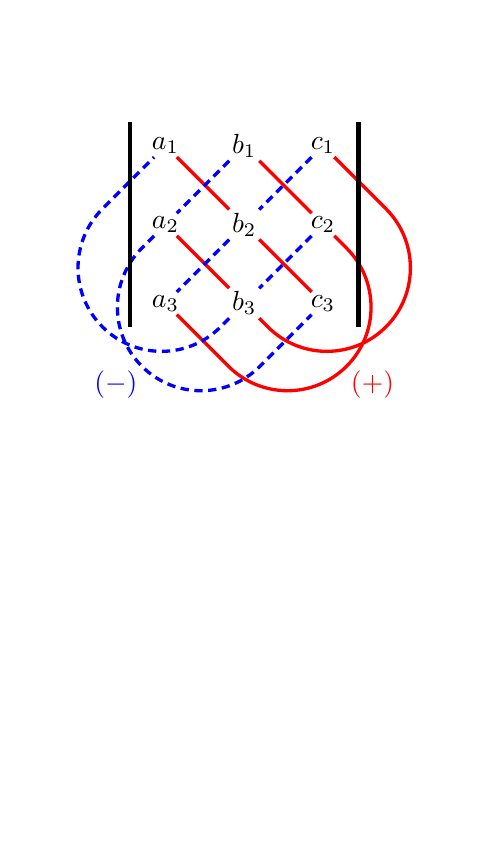
\begin{tikzpicture}[>=latex,scale=0.5,inner sep=1pt]
  \useasboundingbox(-1.5,1)rectangle(9.5,-19);
  \foreach \x in {1,2,3}
  {
    \foreach \y[count=\i] in {a,b,c}
    {\node(\y\x) at (2*\i,-2*\x) {$\y_\x$};}
  }
  \draw[very thick,red](a1)--(b2)--(c3);
  \draw[very thick,red](b1)--(c2)--++(0.6,-0.6)arc(45:-135:{1.5*sqrt(2)})node[midway,below right]{$(+)$}--(a3);
  \draw[very thick,red](a2)--(b3)--++(0.6,-0.6)arc(-135:45:{1.5*sqrt(2)})--(c1);
  \draw[very thick,densely dashed,blue](c1)--(b2)--(a3);
  \draw[very thick,densely dashed,blue](b1)--(a2)--++(-0.6,-0.6)arc(135:315:{1.5*sqrt(2)})node[midway,below left]{$(-)$}--(c3);
  \draw[very thick,densely dashed,blue](c2)--(b3)--++(-0.6,-0.6)arc(315:135:{1.5*sqrt(2)})--(a1);
  \draw[ultra thick] (1.1,-1.4)--(1.1,-6.6);
  \draw[ultra thick] (6.9,-1.4)--(6.9,-6.6);
\end{tikzpicture}
\end{document}